\tikzset{
	node/.style = {circle, draw=black, fill=white},
}

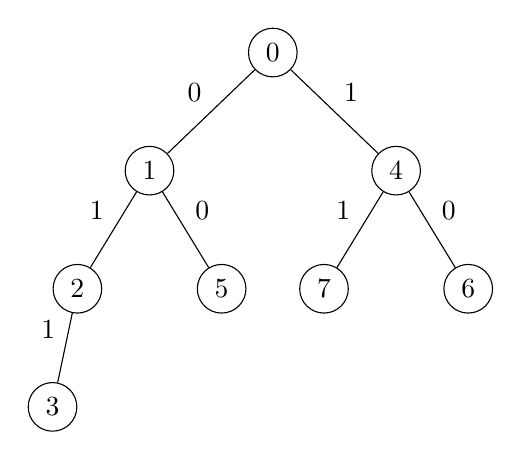
\begin{tikzpicture}
	\tikzstyle{level 1}=[sibling distance=25mm] 
	\tikzstyle{level 2}=[sibling distance=12mm] 
	\node[node]{0}
		child {
			node[node,left]{1}
			child {
				node[node,left]{2}
				child {
					node[node,left]{3}
					edge from parent node [above left] {1}
				}
				edge from parent node [above left] {1}
			}
			child {
				node[node,right]{5}
				edge from parent node [above right] {0}
			}
			edge from parent node [above left] {0}
		}
		child {
			node[node,right]{4}
			child {
				node[node,left]{7}
				edge from parent node [above left] {1}
			}
			child {
				node[node,right]{6}
				edge from parent node [above right] {0}
			}
			edge from parent node [above right] {1}
		}
	;
\end{tikzpicture}
